\documentclass{boi2014-lv}

\usepackage{enumitem}
\usepackage{tikz}
\usepackage{todonotes}
\usepackage{wrapfig}

\renewcommand{\DayNum}{2}
\renewcommand{\TaskCode}{demarcation}
\renewcommand{\TaskName}{Sadalīšana}
\renewcommand{\TaskVersion}{1.2}

\newcommand{\constant}[1]{{\tt #1}}

\begin{document}
    \begin{wrapfigure}{r}{3cm}
        \vspace{-24pt}
		\includegraphics[width=3cm]{\TaskCode.jpeg}
	\end{wrapfigure}

		Ilgu laiku Baitopijas salā valdīja taisnīgais karalis Baitezars, bet pēc viņa pēkšņās nāves viņa divi dēli Baitons un Bitons nevarēja vienoties kurš no tiem mantos troni. Viņi izlēma sadalīt salu divās provincēs un valdīt neatkarīgi.
    %For a long time the island of Bytopia was ruled by the fair king
    %Byteasar. But after the sudden death
    %of the king, his two sons -- twins Biteon and Byteon -- could
    %not come to an agreement which one of them should ascend the throne.
    %Therefore they decided to divide the island into two provinces to
    %rule them independently.  
 
		Uz tasnstūrveida kartes uzzīmētā Baitopijas kontūra ir daudzstūris ar $N$ virsotnēm. Katra daudzstūra mala ir paralēla kartes malai un katras divas secīgas malas ir perpendikulāras viena otrai. %Katrai daustūra malai vienīgie kopīgie punkti ir ar blakus malām.
Katra daudzstūra mala nekrusto un nepieskaras nevienai citai malai izņemot iepriekšējo un nākamo malu.

Bitons and Baitons grib sadalīt daudzstūri divos vienādos daudzstūros ar vienu taisnes nogriezni, kas paralēls kartes malai (Divi daudztūri tiek uzskatīti par vienādiem, ja vienu rotējot, spoguļojot un pārbīdot var pārveidot par otru). Daudzstūra virsotņu un sadalošā nogriežņa virsotņu koordinātas ir veseli skaitļi. 
    %On a map Byteotia is shaped as a polygon of $N$ vertices. Every
    %side of the polygon is parallel to a side of the map, and every
    %two consecutive sides are perpendicular to each other.  Biteon
    %and Byteon want to divide the polygon into two congruent figures,
    %using one line segment contained in the polygon and parallel to a
    %side of the map.  (Two figures are congruent if one can be transformed
    %into the other using a combination of reflections, rotations and
    %translations.) Coordinates of the polygon vertices and the end points
    %of the dividing segment are integers.  
 
		Karaļa dēli Jums prasa noskaidrot vai šāda sadalīšana ir iespējama.
    %The king's sons asked you to verify whether such a division is
    %possible.

    \Task
		
		Dotai salas kontūrai noteikt vai to ir iespējams sadalīt ar vertikālu vai horizontālu nogriezni divos vienādos daudzstūros. Ja tas ir iespējams, tad jāatrod šis nogrieznis.
		%Given the shape of the island, determine if it can be partitioned
    %by a horizontal or vertical segment into two congruent pieces. If
    %it can, find one such segment.

    \Input
		
		Ievaddatu pirmajā rindā rakstīts viens vesels skaitlis $N$, kas norāda daudzstūra virsotņu skaitu. $i$-tajā no nākamajām $N$ rindām rakstīts veselu skaitļu pāris $X_i$ un $Y_i$ ($0 \le X_i, Y_i \le 10^9$), kas atdalīti ar tukšumu un kas norāda $i$-tās virsotnes koordinātas. Virsotnes ir dotas apstaigāšanas secībā, tas ir nogriežņi $(X_1,Y_1) - (X_2,Y_2)$,
    $(X_2,Y_2) - (X_3,Y_3)$, \ldots, $(X_{N-1},Y_{N-1}) - (X_N,Y_N)$ un
    $(X_N,Y_N) - (X_1,Y_1)$ ir daudzstūra malas. Apskatot jebkuras divas secīgas daudzstūra malas tās ir perpendikulāras savā starpā.

	%The first line of the input contains a single integer $N$, the number of
	%vertices. The $i$th of the next $N$ lines contains a pair of integer $X_i$
	%and $Y_i$, separated by space, which are the coordinates of the $i$th
	%vertex.
    %\todo{In what order are vertices given?}

	\Output
	
		Jūsu programmai jāizvada viena rinda. Ja ir iespējams sadalīt salu divās vienādās daļās ar horizontālu vai vertikālu nogriezni, kura galapunkti ir $(x_1, y_1)$ un $(x_2, y_2)$, tad izvadiet 4 veselus skaitļus $x_1$, $y_1$, $x_2$ un $y_2$, kas atdalīti ar tukšuma simbolu. Jābūt spēkā vai nu $x_1 = x_2$ vai arī $y_1 = y_2$. Sadalošajam nogrieznim jāatrodas daudzstūra iekšpusē un tikai tā galapunkti pieskaras daudzstūra malām.
	%Your program should output a single line. If it is possible to divide the
	%island into congruent parts with a horizontal or vertical segment, which
	%endpoints are $(x_1, y_1)$ and $(x_2, y_2)$, print 4 integers $x_1$,
	%$y_1$, $x_2$ and $y_2$, separated by spaces.
	%Either $x_1 = y_1$ or $y_1 = y_2$ must hold.

	%If a suitable division cannot be found, output a single word
	%``\constant{Impossible}'' (without quotes).
	Ja nav iespējams sadalīt izvadiet	\constant{NO}.

    \Examples
	\example
	{
		10 \newline
		0 0 \newline
		1 0 \newline
		1 1 \newline
		3 1 \newline
		3 5 \newline
		2 5 \newline
		2 3 \newline
		1 3 \newline
		1 2 \newline
		0 2
	}
	{
		1 2 3 2
	}
	{
		%This is not the only correct choices of parameters.
		Ievērojiet, ka 3 2 1 2 arī ir derīgs atrisinājums.

        \begin{center}
            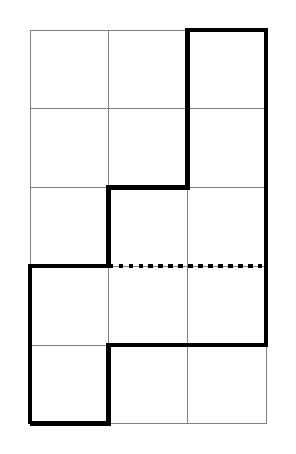
\begin{tikzpicture}
            \draw[help lines] (0,0) grid (3,5);
            \draw[ultra thick] (0,0) -- (1,0) -- (1,1) -- (3,1) -- (3,5) --
                         (2,5) -- (2,3) -- (1,3) -- (1,2) -- (0,2) -- (0,0);
            \draw[ultra thick,dotted] (1,2) -- (3,2);
            \end{tikzpicture}
        \end{center}

	}

	\example
	{
		6 \newline
		0 0 \newline
		1 0 \newline
		1 1 \newline
		2 1 \newline
		2 2 \newline
		0 2
	}
	{
		NO
	}
    {
        Šajā gadījumā nav iespējams sadalīt divās vienādās daļās.
%There is no way to divide the island in this case.
        \begin{center}
            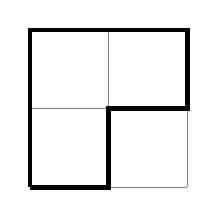
\begin{tikzpicture}
            \draw[help lines] (0,0) grid (2,2);
            \draw[ultra thick] (0,0) -- (1,0) -- (1,1) --
                         (2,1) -- (2,2) -- (0,2) -- (0,0);
            \end{tikzpicture}
        \end{center}
    }


    \Scoring

    \begin{description}
        \item[Apakšuzdevums 1 (12 points).] $4 \le N \le 100\ 000$.
	Jebkura horizontāla vai vertikāla taisne, kas krusto daudzstūri, sadala to tieši divās daļās.
        %Any horizontal or vertical line that divides the polygon divides it into
        %exactly two parts.

        \item[Apakšuzdevums 2 (15 points).] $4 \le N \le 200$
        \item[Apakšuzdevums 3 (23 points).] $4 \le N \le 2\ 000$
        \item[Apakšuzdevums 4 (50 points).] $4 \le N \le 100\ 000$
    \end{description}

    \Constraints

    \begin{description}
        \item[Laika ierobežojums:] 0.5 s.
        \item[Atmiņas ierobežojums:] 256 MB.
    \end{description}

\end{document}
